
\documentclass[11pt]{article}

\usepackage{ifpdf}
\usepackage{xspace}
\usepackage{listings}
\lstset{
  frame=none,
  xleftmargin=2pt,
  belowcaptionskip=\bigskipamount,
  captionpos=b,
  escapeinside={*'}{'*},
  language=haskell,
  tabsize=2,
  emphstyle={\bf},
  commentstyle=\it,
  stringstyle=\mdseries\rmfamily,
  keywordstyle=\bfseries\rmfamily,
  columns=flexible,
  basicstyle=\small\sffamily,
  morecomment=[l]\%,
}
\ifpdf 
    \usepackage[pdftex]{graphicx}   % to include graphics
    \pdfcompresslevel=9 
    \usepackage[pdftex,     % sets up hyperref to use pdftex driver
            plainpages=false,   % allows page i and 1 to exist in the same document
            breaklinks=true,    % link texts can be broken at the end of line
            colorlinks=true,
            pdftitle=My Document
            pdfauthor=My Good Self
           ]{hyperref} 
    \usepackage{thumbpdf}
\else 
    \usepackage{graphicx}       % to include graphics
    \usepackage{hyperref}       % to simplify the use of \href
\fi 
\graphicspath{ {images/} }

\title{Report}
\author{Giovanni Garufi}
\date{}

\begin{document}  

\newcommand{\diff}{\texttt{diff3}\xspace}
\newcommand{\SOP}{SOP\xspace}
\newcommand{\alins}{\texttt{Alins}\xspace}
\newcommand{\aldel}{\texttt{Aldel}\xspace}
\newcommand{\alspn}{\texttt{Alspn}\xspace}
\newcommand{\scp}{\texttt{Scp}\xspace}
\newcommand{\scns}{\texttt{Scns}\xspace}
\newcommand{\schg}{\texttt{Schg}\xspace}

\maketitle

\section{Introduction}
Version control systems (VCS) have been steadily becoming an ubiquitous and central 
tool in programming. Many big projects, with hundreds of collaborators, 
fundamentally rely on these kind of tools to allow collaborators to interact 
with one another and to keep a structured log of the units of change. 
At the heart of most modern VCS is the unix diff utility. This tool computes a 
line-by-line difference between two files of text, determining the smallest set 
of insertions or deletions of lines that transform one file into the other. This sequence of transformation 
produced by \diff is called an edit script. 
When two collaborators have modified the same source file in independent 
ways and the VCS wants to reconcile the two independent changes into a single 
one it will attempt to produce an single edit script that encompasses both changes, this is commonly referred to 
as a merge. This operation is clearly not always possible: if two collaborators have 
modified the same line the two resulting edit scripts will 
``overlap'', it is not clear which one of the two modifications should be 
picked.  

In general, some conflicts will always require a manual intervention: when two 
people change the same thing in two different ways there is no general way of 
deciding which should be the resulting transformation; however the diff tool makes 
a big assumption in considering lines to be the basic units in which change is 
observable.  

According to diff, two unrelated changes on the same line would still give rise to a 
conflict that requires manual intervention. 
The main idea of this research is to design an alternative to diff which offers a 
finer grained control over the units of change. By attempting to extend the diff algorithm to operate on an AST that 
represents the parsed program we are able to focus on smaller units of change, this allows us to produce 
more accurate patches. 

The drawback of this approach is that it moves the problem from the 
world of strings to the world of trees, and the problem of computing a patch between two elements suddenly
becomes computationally more expensive. 
Approaches similar to this one have already been explored in previous literature
\cite{semantics-VC}, \cite{structure-aware-VC} and \cite{vassena}. In these works, the problem of computing 
the difference between two trees was always reduced to the problem of computing the difference of a flattened
representation of the tree. While the flattened representation makes the problem of computing a difference 
easier,
it makes reconstructing a valid tree from the representation more complex, and patches are more likely to 
generate ill-structured data.  The novelty in the work of Miraldo, Dagand and Swierstra \cite{type-directed-diff} 
lies in the idea of enforcing a structure-preserving, type-directed approach. On 
one hand structural information is directly encoded in the patches, so that applying a patch will always produce well formed code. On 
the other hand, the type information encoded in the grammar of the AST is 
exploited in the creation of a patch, making the process more efficient.

The paper introduces a theoretical and practical framework to define and compute patches between 
structured data. This framework is generic and makes extensive use of dependent 
types in order to guarantee structure preserving transformations.

\section{Overview}\label{overview}
In the remainder of this proposal we will show a full Haskell implementation of the algorithm presented by Miraldo 
et al. \cite{type-directed-diff}, which is presented in Agda in the original paper. 
The algorithm is implemented generically and described with dependent types; in 
order to perform experiments I ported the implementation to Haskell. Haskell is scheduled to land full support 
for dependent types in the next couple of years \cite{dependent-haskell}, in the meanwhile, they can only 
be partially supported through some ad-hoc techniques. Both Generics and Dependent Types require some language 
extensions and machinery which are non trivial in Haskell: for this reason some time is spent introducing the
techniques and setting up the building blocks for the implementation. 

The following section is an introduction to dependent types in Haskell as they will be crucial in encoding 
the structure we want to express in our data types and their transformations. 
Essentially we want to characterise patches by the transformation they operate 
on the source code (e.g. the patch that adds an extra argument to a function) as 
such we need dependent types to reflect onto the type system the action of a 
patch on a certain value. This will assure that any code produced by the 
algorithm is structurally valid by construction.

 Following dependent types we will need to introduce sums of products: these give us a general way to view 
types and will allow us to define an algorithm that is independent of the representation of the AST for the language 
we are treating. In this regard there is a fine balance between having a core algorithm which is generic and can 
be applied to any language, and the use of domain-specific strategies to guide the generation of patches by using 
knowledge specific to the language in question. One of the goals of this thesis is to investigate this balance: 
how necessary are domain-specific differencing strategies in order to keep the combinatorial explosion in check? 
Despite the generality of the algorithm, we have instantiated it for the Clojure programming language 
\cite{clojure}; this choice is motivated by the general simplicity of parsing languages that derive from 
LISP and by the need to select a language that is popular enough to have large 
active projects, available on Github, that will provide us a good sample of data 
to test.

In the last sections we will review some of the possible 
future directions that can be explored with this framework both in terms of 
gathering concrete evidence about the performance of the algorithm and extending 
it in order to explore the different design choices that were made along the way.

\section{Dependent types in
Haskell}\label{dependent-types-in-haskell}

With time, Haskell's type system has kept evolving from its humble
Hindley-Miller origins and through the use of different language extensions it has gained the ability 
to express more complex types. In particular, many efforts have gone to add partial support for dependently
typed programming in the latest years.

One major stepping stone in this direction is the DataKinds (\cite{datakinds}) extension which duplicates an ordinary data type, such as

\begin{lstlisting}[language=haskell]
data Nat = Z | S Nat
\end{lstlisting}

at the kind level, this means that from this declaration we automatically get two new types, namely \texttt{Z} of kind \texttt{Nat}
and \texttt{S} of kind \texttt{Nat\ -\textgreater{}\ Nat}.

We can use the \texttt{Nat} kind to index generalised algebraic data
types (GADTs) in a way that allows us to create an analogue of a
dependent type. In the case of \texttt{Nat}, we can use it to define a
GADT for vectors of a given length.

\begin{lstlisting}[language=haskell]
data Vec :: * -> Nat -> * where
  Vn ::                   Vec x Z
  Vc :: x -> Vec x n -> Vec x (S n)
\end{lstlisting}

Such a vector is either the empty vector, which is indexed by
\texttt{Z}, or a vector which is built by adding an element of
type \texttt{x} in front of a vector of \texttt{xs} of length \texttt{n},
yielding a vector of \texttt{xs} of length \texttt{S\ n}.

This allows us to define principled analogues of some functions which
operate on lists. The infamous \texttt{head} function will
crash our program when passed an empty list; equipped with these \texttt{Vec}, we can rule this
out by construction. 

This is how we can define a \texttt{head} function on vectors.

\begin{lstlisting}[language=haskell]
head :: Vec x (S n) -> x
head (Vc h t) = h
\end{lstlisting}

Informally, we are saying that the \texttt{head} function takes as
argument a vector with length strictly greater than 0. In this way, if we
try to pass an empty vector to \texttt{head} we will get a compile time
error instead of the usual runtime one.

Another extension which plays a crucial role in dependent types is
\texttt{TypeFamilies}: informally it allows us to write functions which operate on types, 
we will use this to define concatenation between \texttt{Vec}s.

The following type family can be seen as a function that takes two types
of kind \texttt{Nat} and returns another type of kind \texttt{Nat}
representing the result of adding those two types.

\begin{lstlisting}[language=haskell]
type family (m :: Nat) :+ (n :: Nat) :: Nat where
  Z      :+ n = n
  (S m) :+ n = S (m :+ n)
\end{lstlisting}

Equipped with this type family we can now define concatenation between
vectors.

\begin{lstlisting}[language=haskell]
vappend :: Vec x n -> Vec x m -> Vec x (n :+ m)
vappend Vn          ys = ys
vappend (x `Vc` xs) ys = x `Vc` (vappend xs ys)
\end{lstlisting}

One interesting thing to note is that up to this point, we never use the
\texttt{Nat} part of a vector at runtime. That information is only used
at compile time to check that everything ``lines up'' the way it should
be, but it could actually be erased at runtime.

Suppose we want to write a \texttt{split} function, this function takes
an \texttt{n} of kind \texttt{Nat}, a vector of length \texttt{n\ :+\ m}
and splits it into a pair of vectors, with respectively \texttt{n} and
\texttt{m} elements.

The first problem we incur in is that we can not pass something of kind
\texttt{Nat} to our \texttt{split} function, in fact the types \texttt{Z} and \texttt{S} have no inhabitants, so we can
not construct any term of those types. Furthermore, we want to
express that this \texttt{n} of kind \texttt{Nat} that we pass as a
first argument, is the same \texttt{n} as in the vector length. The idea is to 
wrap this type into a singleton data type, giving us a dynamic container of the static 
information.

\begin{lstlisting}[language=haskell]
data SNat :: Nat -> * where
  SZ ::           SNat Z
  SN :: SNat n -> SNat (S n)
\end{lstlisting}

The name singleton comes from the fact that each type level value of
kind \texttt{Nat} (namely \texttt{Z} or \texttt{S} applied to another
type of kind \texttt{Nat}) has a single representative in the
\texttt{SNat} type.

The following figure gives a good representation of this process: the
DataKinds extension promotes things of type \texttt{Nat} to things of
kind \texttt{Nat}. The singleton allows us to take one step back in this
ladder, and associates to every thing of kind \texttt{Nat} a term from
the singleton type \texttt{SNat}. The following picture, borrowed from Eisenberg et al. \cite{singletons}, gives a good 
representation of this process.

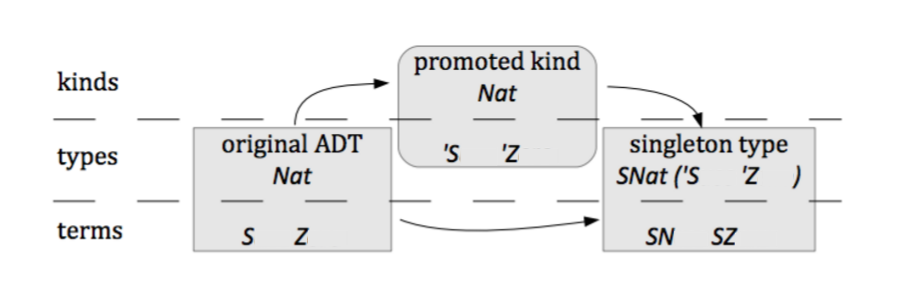
\includegraphics[width=\textwidth]{singleton.png}

We can think of the DataKinds extension as a way of embedding dynamic information into the static fragment of 
the language. Singletons, on the other hand, are a way to reflect this static information back to 
the dynamic level, and make runtime decisions based on the types we obtain.


Singletons solve the two problems outlined above: they have kind \texttt{*}
and contain a \texttt{Nat} that we can later refer to in our
function definition. We can now define \texttt{split} as follows:

\begin{lstlisting}[language=haskell]
split :: SNat n -> Vec x (n :+ m) -> (Vec x n, Vec x m)
split SZ     xs          = (Vn, xs)
split (Sn n) (x `Vc` xs) = (x `Vc` ys, zs)
  where
    (ys, zs) = split n xs
\end{lstlisting}

With these three tricks up our sleeve (data kind promotion, type level
functions and singletons) we can emulate some of the features that are
present in dependently typed languages such as Agda. These features allow us to 
emulate explicit dependent quantification. We can actually go even further in 
Haskell: Lindley et McBride \cite{hasochism} show us how to emulate implicit types via type 
classes and ultimately how all kinds of quantification, modulo some boilerplate, are possible in 
Haskell.

\section{Sum of Products}\label{SOP}


The basic idea of the Sum of Products (SOP) approach is to define a ``normal form'' for all generic representations of data types and 
to define functions that act on this form. It is, in some sense, similar to the Disjunctive Normal Form for propositional logic in the 
sense that every proposition can be expressed in DNF and we can write theorems (functions) 
which assume the expression is represented in DNF.
The bulk idea is to view each type as a choice between a constructor and all the arguments that are passed to
that constructor. It is useful to think about the two different levels: on the first level we 
make a choice about which constructor to pick; this corresponds to a sum
over all the constructors of the type. On the second level, we are choosing a certain number of arguments 
to feed to that constructor and this can be viewed as a list, or product, of 
those arguments. Clearly the products will depend on the choice of constructor, 
each of which could take a different number of arguments of possibly 
different types. This motivates the need to represent the product as some sort 
of heterogeneous list. A constructor can also take no arguments, in which case we 
can simply use an empty list to represent that, but can also take an argument of 
the same type it is trying to construct (like the \texttt{S} constructor from the previous section). 
In this case, the recursive argument can itself be encoded as an SOP 
and the same encoding can be used all the way down to the leaves. 


Since every data type can be encoded as an SOP, we can write functions 
that act on this representation and regard them as generics. For every data type 
we can first convert it to the SOP representation and then pass it to 
the desired function. Since the SOP representation is isomorphic to the original type, we can eventually reconstruct the 
desired term after we are done working with the representation. This encoding is 
presented by Loh et al. \cite{true-sop} and represents one of the numerous different ways to 
approach generic programming in Haskell. 
In the remainder of this section we will try to formalise the intuition presented 
above by building the SOP representation of a data type. 

\vfill

An AST consists of a family of datatypes, with a main one which
represents the outer structure of the language, and a number of other
possibly mutually recursive datatypes appearing as arguments to the
constructors of the main datatype. We can define a very simple language which 
consists of only one datatype, \texttt{SExpr} which is isomorphic to binary trees 
of integers. This choice is just for ease of presentation, the following construction 
can be applied to a family of mutually recursive datatypes.

\begin{lstlisting}[language=haskell]
data SExpr = Operation SExpr SExpr | Value Int
  deriving (Eq, Show)
\end{lstlisting}

For each type that appears as an argument to a constructor in our family
of datatypes, we will construct an atom representing that type.
Following the example above, we will define

\begin{lstlisting}[language=haskell]
data U = KInt | KSExpr 
\end{lstlisting}

Now, we can group all the constructors appearing in our original
datatypes under the \texttt{Constr} type in a similar way as we
did for the atoms. 

\begin{lstlisting}[language=haskell]
data Constr = Operation | Value
\end{lstlisting}

We have now deconstructed our original datatype into two levels: \texttt{Constr} corresponding to the level of sums (the constructor) 
and  \texttt{U} corresponding to the level of products (the atoms).

Since we had to define two additional datatypes that have no relation between 
each other we need a way to tie them together on the type level.
To achieve this, we define the \texttt{ConstrFor} data type,
which can be viewed as a proof that a certain constructor builds element
of a certain family. In general an AST consists of a family of possibly 
recursive datatypes, hence we will need the additional information about what 
family the constructor \texttt{Constr} belongs to.

\begin{lstlisting}[language=haskell]
data ConstrFor :: U -> Constr -> * where
  OperationProof :: ConstrFor KSExpr Operation
  ValueProof     :: ConstrFor KSExpr Value
\end{lstlisting}

Finally we must encode one last bit of information: the ``shape'' of
each constructor. To do so, we can use a closed type family which can be
viewed as a function on types. This function takes a \texttt{Constr} and
returns a list of atoms representing the arguments the constructor
accepts.

\begin{lstlisting}[language=haskell]
type family TypeOf (c :: Constr) :: [U] where
  TypeOf Operation = '[KSExpr, KSExpr]
  TypeOf Value = '[KInt]
\end{lstlisting}

We will also need to associate each atom with a singleton, which will
allow us to relate terms of our language to their type level representation. 

\begin{lstlisting}[language=haskell]
data Usingl :: U -> * where
  Uint    :: Int -> Usingl KInt
  Usexpr  :: SExpr -> Usingl KSExpr
\end{lstlisting}

Since \texttt{TypeOf} returns something of kind \texttt{{[}U{]}} we will
define another GADT named \texttt{All}, that maps a type constructor
\texttt{k\ -\textgreater{}\ *} over an argument of kind \texttt{{[}k{]}}
giving us something of kind \texttt{*} to quantify over a list of singletons.

The definition for \texttt{All} is straightforward:

\begin{lstlisting}[language=haskell]
data All (k -> *) :: [k] -> * where
  An :: All p '[]
  Ac :: p x -> All p xs -> All p (x ': xs)
\end{lstlisting}

With this setup we can finally construct the \texttt{View} datatype;
this loosely corresponds to a generic view as sum of products of a
datatype, and simply deconstructs each term of a type into a constructor
and a list of arguments applied to that constructor

\begin{lstlisting}[language=haskell]
data View u where
 Tag :: ConstrFor u c -> All Usingl (TypeOf c) -> View u
\end{lstlisting}

An element of type \texttt{View u} represents an element of type \texttt{u} 
deconstructed into its SOP view; the first argument records the choice 
of the constructor for that datatype and the second is the heterogenous list of 
arguments that are required to build that constructor, note that we are 
dependently relating the shape of the product to the actual choice of 
constructor (the \emph{c}).

To conclude the section we can attempt to construct the \texttt{View} of a 
simple expression representing an operation between two values.

\begin{lstlisting}[language=haskell]
  expr = Operation (Value 1) (Value 1)
\end{lstlisting}

The outmost constructor (\texttt{Operation}) gets mapped to the corresponding 
\texttt{OperationProof}; the shape of the second 
argument ($[KSExpr, KSExpr]$) is completely determined by 
this choice.

\begin{lstlisting}[language=haskell]
  viewExpr = Tag OperationProof (Usexpr (Value 1) `Ac` Usexpr (Value 1))
\end{lstlisting}

Constructing a view can be thought as a way to unwrap the top-most level of the 
AST; as shown in the example above, the values of the operation are left untouched in 
the resulting view. Loosely speaking this justifies the intuition that 
viewing a type as a sum of products gives us information about its shape but 
does not change any information about its values, enabling us to switch back and 
forth between representation without losing anything.


\section{Type-directed diff}\label{type-directed-diff}

The approach presented by Miraldo and Swierstra \cite{type-directed-diff} takes advantage of the structure 
encoded in types to define a generic type-directed diff algorithm between
typed trees. The inspiration comes from the diff utility present in
Unix which is at the heart of the current methodologies employed by VCS
to attempt to compute a patch between two different versions of the same
file. The limitations of the diff algorithm, as it currently stands, is
that it does not employ any structural information about the data it is trying to calculate a patch on. 
Files are parsed on a line by line basis and, as the authors show, this is somewhat resilient to vertical changes in the
source code. On the other hand it completely breaks down when dealing with horizontal
changes, which constitute a heavy chunk of the changes that are usually
made to code.

Suppose we have the following innocuous looking function in clojure:

\begin{lstlisting}[language=lisp,numbers=left]
(defn head [l]
  (first l))
\end{lstlisting}

Suppose we make two independent modifications, the first of which adds a default 
parameter to be returned in case the list is empty, and the second one that 
changes the name of the function from \emph{head} to \emph{fst}.

\begin{lstlisting}[language=lisp,numbers=left]
(defn head [l, d]
  (if (nil? l)
    (d)
    (first l)))
\end{lstlisting}

\begin{lstlisting}[language=lisp,numbers=left]
(defn fst [l]
  (first l))
\end{lstlisting}

When attempting to reconcile these two changes with the diff algorithm we will run into problems.
Despite the two are modifying disjoint pieces of the 
actual code, the diff algorithm employed by most VCS when trying to 
compute a merge patch between three objects will output a conflict. 
The reason is that both changes touch the same line; this is a nuisance in  
terms of having to manually solve the conflicts. Furthermore it also 
introduces some level of non-determinism, as the presence of conflicts may depend on 
things like indentation instead of being a fundamental property of the 
transformation. 

The underlying idea to the approach presented in the article is to employ
the generic SOP view presented in the preceding section to define a
generic way to view datatypes. Once that is settled, we obtain a view of
any well defined program as a structured tree of data, where each object
we inspect can be represented as a choice of a certain constructor,
among the available ones, and a choice of arguments to that constructor.

In the process of transforming one tree into another we need to keep track of three different things: 
\begin{itemize}
  \item Changes on the constructor level - The internal nodes of the trees
  \item Changes on the product level - The branches that go from a node to its children
  \item Changes on the atoms - The elements that are pointed to by the branches
\end{itemize}

The atoms can be either other internal nodes, in which case we recurse down the 
tree, or leaves in which case we record the pair of source and target leaf.

We will use the simple binary tree language presented in previous sections as a 
working example to show the construction of a patch. The transformation we will walk through is the following:
given the following AST:
\begin{lstlisting}[language=haskell]
p1 = Operation (Value 1) (Operation (Value 1) (Value 1))
\end{lstlisting}
we want to characterise the patch that transforms it to 
\begin{lstlisting}[language=haskell]
p2 = Operation (Value 1) (Operation (Value 2))
\end{lstlisting}

The first structure we will employ is the \emph{spine}, this can be thought of as a common skeleton between 
the two trees which captures the parts that do not change under the transformation.

\subsection{Spine}\label{spine}

We will define Spines to only between two elements of the same sum-type, and defer to later the discussion on how
to perform transformation between elements of different sum-types. Calculating a spine for two elements of the same sum-type 
loosely corresponds to calculating the longest common prefix between two strings. Recall that the two 
elements \emph{x} and \emph{y} are viewed as SOP, in this sense calculating the
spine between \emph{x} and \emph{y} corresponds to capturing the common
coproduct structure between them. Let $x$ and $y$ be two such elements, we will have three cases to
consider. 
\begin{itemize}
  \item $x = y$
  \item $x$ and $y$ have the same constructor on the sum level but differ in the 
  arguments
  \item $x$ and $y$ have different constructors
\end{itemize}

This gives rise
to the following three different constructors for the Spine GADT, each
corresponding to one of the cases described above.

\begin{lstlisting}[language=haskell]
data Spine (at :: U -> *)(al :: [U] -> [U] -> *) :: U -> * where
  Scp  :: Spine at al u
  Scns :: ConstrFor u s -> All at (TypeOf s) -> Spine at al u
  Schg :: ConstrFor u s -> ConstrFor u r
       -> al (TypeOf s) (TypeOf r)
       -> Spine at al u
\end{lstlisting}

If the two
elements are the same, the spine is a copy. If the top level
constructors match, the spine consists of this information and a function to
transform the pairs of constructor fields. Lastly, if two constructors
don't match, the spine must record this and also contain a function to
transform the list of source fields into the list of destination fields.
\\\\
The \texttt{Scp} constructor corresponds to the first case, in which we need
to record no additional information other than the fact that the two
elements are equal. 
Before looking at the other two constructors, let us focus our attention for a moment to the three arguments that a spine takes:
the third parameter of the spine (the \texttt{U}) represents the
underlying type for which we are trying to compute a patch, the sum-type to which $x$ and $y$ both belong.
The other two, \texttt{al} and \texttt{at} are respectively a
function between products that describes what to do with the different
constructor fields and a function between atoms which describes what to
do with the paired fields in case we have the same constructor.
These functions are needed for the remaining constructors: the \texttt{Scns} constructor corresponds to the 
case where the constructor is left untouched but some of the arguments have changed.
For this reason its second argument consists of the predicate \texttt{at} applied to the list of arguments which describes
how to transform them. 

Finally, \texttt{Schg} represents a change of constructor on the sum level: the first two arguments record the
source and destination constructors, the third argument is the
\texttt{al} function applied to the constructor fields of the source and
destination constructor respectively.

Let's not worry about the \texttt{al} and \texttt{at} parameters for the time 
being, these will later be used to close the recursive knot and generate the full patch by interleaving
the construction showed here and in the following sections. 
For now we can simply observe that if we were to calculate a spine between the 
two programs introduced above we would proceed by constructing their view as 
presented in \ref{SOP} obtaining the following

\begin{lstlisting}[language=haskell]
p1 = Tag OperationProof (Usexpr (Value 1) `Ac` Usexpr (Operation (Value 1) (Value 1)))
p2 = Tag OperationProof (Usexpr (Value 1) `Ac` Usexpr (Value 2))
\end{lstlisting}

These views are not completely equal, but their first argument is. This represents the outer choice 
of constructor and we are after all ultimately transforming an \texttt{Operation} into another one. The spine produced
by these two views will then start with an \texttt{Scns} recording the fact that 
the outer constructor has stayed the same but there are some changes in its 
arguments.

\begin{lstlisting}[language=haskell]
spine = Scns OperationProof _
\end{lstlisting}

We ignored the second argument up to this point (representing it as an underscore); let's turn our attention to 
that now: since we know that the constructor is unchanged in the transformation, we also know that 
both for the source and destination tree, the number and types of its arguments 
will be the same. For this reason we can simply pair up the corresponding 
arguments and calculate the diff between every pair. The second argument to \texttt{Scns} can be read as: the function 
\texttt{at} applied to a list of pairs of elements of the same type. The type of each 
pair is specified by \texttt{TypeOf s}, which in our working example is equal to 
$[Usexpr, Usexpr]$. Essentially we have a list of \texttt{Usexpr} pairs and are 
left with the problem of calculating patches between the elements contained in 
each pair. 
We can easily see that the first pair of our example will give rise to an 
\texttt{Scp}, the two subtrees are in fact the same and we can simply copy the 
information along the transformation. The second pair is more interesting 
though: this is the case where we have a change on the constructor level and the 
spine we produce will be the following
\begin{lstlisting}[language=haskell]
  Schg OperationProof ValueProof _
\end{lstlisting}
However the remaining argument to fill is not as simple as the \texttt{Scns} 
case since \texttt{Operation} and \texttt{Value} expect completely different 
arguments.
In the case where the constructor had remained the same, we could 
pair up the arguments and proceed from there; however, when the
external constructor has changed, there is no obvious way of pairing up
the arguments. Indeed they might be completely in different numbers and types, which 
motivates the following definition of alignments.

\subsection{Alignment}\label{alignment}

The spine takes care of matching
the constructors of two trees, alignments handle the products packed within the constructors.
Recall that this alignment has to work between two heterogeneous lists
corresponding to the fields associated with two distinct constructors.
The approach presented below is inspired by the existing algorithms
based on the edit distance between two strings. The problem of finding
an alignment of two lists of constructor fields can be viewed as the
problem of finding an edit script between them. An edit script is
simply a sequence of operations which describes how to change the source
list into the destination. In the case of \diff the source and destination lists are the lists of lines in the source and destination files; in our context
the source and destination lists are the products of fields of the source and destination constructors respectively. 
To compute an edit script we simply
traverse the lists, from left to right, considering one element from each
list. At each step we are presented with three choices:

\begin{itemize}
\item
  We can match the two elements (Amod) of the list and continue
  recursively aligning the rest
\item
  We can insert the destination element before the current element in
  the source list (Ains) and recursively compute an alignment between
  whatever we have in the source list and the tail of the destination.
\item
  We can delete the element from the source list (Adel) and recursively
  compute the alignment between the rest of the source and the
  destination.
\end{itemize}


The following GADT models the sequence of operations that represent an 
alignment.

\begin{lstlisting}[language=haskell]
data Al (at :: U -> *) :: [U] -> [U] -> * where
  A0   :: Al at '[] '[]
  Ains :: Usingl u -> Al at xs ys -> Al at xs (u ': ys)
  Adel :: Usingl u -> Al at xs ys -> Al at (u ': xs) ys
  Amod :: at u -> Al at xs ys -> Al at (u ': xs) (u ': ys)
\end{lstlisting}

\texttt{Al} is parametrised by the same type-level function introduced in the spine. 
\texttt{A0} represents the empty alignment, \texttt{Ains} and \texttt{Adel} take as first argument
a singleton representing the element being inserted or deleted. These two, together
with an alignment for the rest of the list, give us the alignment with
an insertion (resp. deletion) as explained in the section above. In the
\texttt{Amod} case the first argument is the predicate on the underlying atom that describes how to transform 
it and the second one, as for the case of insertions and deletions, represents an  
alignment between the rest of the lists. 

One key difference to keep in mind, between the edit scripts produced by diff and the alignments is the atomicity 
of the elements being aligned (lines and sub-trees respectively). In the
case of strings we can assume deletions and insertions to be somewhat
equivalent in cost thus we can safely try to maximise one of the two.
However, in our case, the elements we are inserting or deleting are
sub-trees of arbitrary size, therefore it is not obvious if we should try and maximise
insertions or deletions.

This poses the problem that when enumerating alignments we have no guiding heuristic to cut the number
of solutions, for the time being we will simply ignore the problem and resort to enumerate
all possible alignments, avoiding to skew the algorithm into preferring
insertions over deletions or vice versa.

Let's walk through calculating the alignment for our running example: we have to 
produce an alignment between \texttt{[KSExpr, KSExpr]} and \texttt{[Kint]} (recall that these are the shapes of the 
\texttt{Operation} and \texttt{Value} constructors). Because of the way we 
define the \texttt{Amod} constructor, more precisely because of the \texttt{at} 
function that describes how to transform an atom into the other we restrict 
ourselves to only attempt an \texttt{Amod} between two singletons of the same underlying 
type. This means that in a case like this one, we will only be able to transform 
one list into the other by repeated applications of \texttt{Ains} or 
\texttt{Adel}. It is worth noticing that this restriction is not mandatory and 
we could in principle allow these transformations as well, the choice here is purely pragmatical and the underlying reason is,
this will be a recurring theme, to reduce the sheer amount of combinations that must be checked.
What we are left with are the three possible alignments that can be formed by inserting the \texttt{Uint}
and deleting the two \texttt{Usexpr}s, we will generate all of them and keep performing 
the computations on each branch. 

\subsection{Atoms}\label{atoms}

Having figured out all the alignments between two lists of constructor
fields, we still have to decide what to do in the case where we match two
elements. We need to make a distinction between the possibly
recursive fields and the constant ones.
In the case of constant fields
like \texttt{Int}s or \texttt{String}s, a transformation between two
values of this type consists of a pair recording the source value and the
destination value. In the case of a recursive datatype we are
essentially left with the problem we started from: transforming a value
of a data type into another. To do so, we simply start all over again,
recursively computing a spine and an alignment between constructor
fields. Note that this construction explicitly excludes pairing constant atoms 
to recursive ones, this choice serves to prune the search space and reduce the 
number of possible pairings that can be constructed.
\\\\
To represent pairs of constant atoms we introduce a helper \texttt{Contract} datatype which 
lifts f over a pair of xs.

\begin{lstlisting}[language=haskell]
  newtype Contract (f :: k -> *) (x :: k) = Contract { unContract :: (f x , f x) }
\end{lstlisting}

To distinguish between recursive and non recursive elements of the language we 
define a typeclass with no additional methods, and add instances of this typeclass only for the recursive atoms.

Once again, borrowing the language definition from the previous section, we will have the following 
class and instances defined
\begin{lstlisting}[language=haskell]
class IsRecEl (u :: U) where
instance IsRecEl KSExpr where
\end{lstlisting}

With this we can define the following datatype to represent diffs between atoms of our language.
\begin{lstlisting}[language=haskell]
data At (recP :: U -> *) :: U -> * where
  Ai :: (IsRecEl u) => recP u -> At recP u
  As :: Contract Usingl u -> At recP u
\end{lstlisting}

Here the \texttt{At} datatype is parametrised by a predicate that describes how 
to transform the recursive atoms. 
The first constructor, \texttt{Ai}, which represents the recursive case is 
parametrised by this predicate, the constraint is added to ensure by construction 
that when we build an \texttt{Ai} we can only do so for the elements of the 
language that actually are recursive.
The other case is covered by the \texttt{As} constructor, recall that in this case \texttt{Contract} simply lifts 
\texttt{Usingl} to a pair of elements of type \emph{u}, so the first parameter 
can be read as: a pair of \texttt{Usingl u}.

In our example we have already seen the case for \texttt{Ai}, the atoms paired 
by the first spine were all \texttt{Kexpr}s which we recursively calculated spines on. 
The \texttt{As} will be produced when we match two \texttt{Value}s that contain 
different integers, in that case we produce a pair of \texttt{Usingl Kint} that record 
the transformation from one \texttt{Int} to the other.

\subsection{Recursive alignments}\label{recursive alignments}

Starting by computing the spine is not necessarily the optimal choice, this can 
be seen from the following simple example between lists:

\begin{lstlisting}[language=haskell]
  [ 1, 2, 3, 4 ] -> [ 2, 3, 4 ]
\end{lstlisting}
Clearly the optimal patch will proceed to delete the first element and then 
copy over any remaining one. Our definition, however, does not allow for such 
deletions. Deletions (resp. insertions) are only handled by alignments. To 
handle such cases we can extend our spines and alignments with the datatype 
\texttt{Almu} that allows insertions or deletions to happen at the top-level.

A match of constructors will be represented as a spine while insertions and 
deletions will record the constructor being inserted (resp. deleted) and a 
\texttt{Ctx} which records which fields are associated to that constructor.
\texttt{Ctx}s list zippers \cite{zippers}: they can be thought as a representation 
of a type with a hole somewhere; the hole represents the place where we 
plug in the rest of the tree to continue the computation.
\begin{lstlisting}[language=haskell]
data Almu :: U -> U -> * where
  Alspn :: Spine (At Almu) (Al (At Almu)) u -> Almu u u
  Alins :: ConstrFor v s -> Ctx (Almu u) (TypeOf s) -> Almu u v
  Aldel :: ConstrFor u s -> Ctx (Almu v) (TypeOf s) -> Almu u v
\end{lstlisting}

This gives rise to another occasion for non-determinism, as \texttt{Almu} has 
the same shortcomings of \texttt{Al} meaning that we have no obvious choice of 
what operation should be maximised over the others. As for alignments we decide to proceed non-deterministically
and compute every possibly choice, the next section will introduce some possible optimisations 
that can be carried out on these two levels to reduce the number of branches 
being generated at each step.

\subsection{Putting everything together}\label{putting everything together}

We can write this function from the ``bottom up'',
starting from the atoms and working our way up through spines and recursive alignments. 
Notice how all these functions return a list of results, as non-determinism 
comes into play at every step. The signatures have been slightly simplified from 
the actual implementation where, for example, the result is 
parametrised by a monad, making it more general.
The diff function for atoms should have the following signature
\begin{lstlisting}
  diffAt ::  (forall r . IsRecEl r => Usingl r -> Usingl r -> [rec r])
            -> Usingl a -> Usingl a -> [At rec a]
\end{lstlisting}
This function is parametrised by a function that describes the treatment for 
recursive atoms. By inspecting the first singleton we learn whether the atom is 
recursive or not; if that is the case, the function that deals with the 
recursive elements can be used to build the corresponding \texttt{At}. In the 
other case, when the element is non recursive, we can simply pair up the two 
constant atoms with a \texttt{Contract} and build the non recursive \texttt{At}.

We can then proceed by implementing the function that computes all the spines 
between recursive elements.
\begin{lstlisting}
 diffS :: IsRecEl a => (forall r . IsRecEl r => Usingl r -> Usingl r -> [rec r])
        -> Usingl a -> Usingl a -> [Spine (At rec) (Al (At rec)) a]
\end{lstlisting}
\texttt{diffS} lifts the parameter it takes, a function to handle the 
recursive elements of our language, over the predicate parameters to the spine that results 
from the two singletons.

We finally have to define a function that computes the diff in terms of 
\texttt{Almu}s. This will call \texttt{diffS} in case of two matching constructors from which we can compute
the spine wrapping that with the corresponding \texttt{Alspn} constructor. In the other cases it will 
attempt the insertion (resp. deletion) at the constructor level by recording the constructor being inserted
(deleted) and producing a \texttt{Ctx} which describes where the original tree is attached in respect to
the added (deleted) constructor.
This function will have the following signature

\begin{lstlisting}
  diffAlmu :: (IsRecEl u, IsRecEl v) => Usingl u -> Usingl v -> [Almu u v]
\end{lstlisting}

As is the case for the alignment between products, here we will simply proceed 
by enumerating all possible recursive alignments, attempting at each level 
the alignment of spines, insertions and deletions.
One shortcoming with this approach lies in the great combinatorial 
explosion of possibilities that arises in computing the alignments for 
constructors and products. The following paragraph will describe an  
we can employ to prune the number of possible alignments. This optimisation 
will allow the program to run in an acceptable time in real world scenarios, however 
we are still at least an order of magnitude slower than \texttt{diff3}, this points to 
the necessity of further and more aggressive optimisations that may be explored 
in future work.

\paragraph{Optimisation}\label{optimisations}

Given the \texttt{Al} and \texttt{Almu} type defined in the previous paragraphs we are still left with the problem
to computing these two levels of alignments. Since we don't know a priori which alignment
is more efficient we will non-deterministically compute all the possible ones. The number of all possible alignments  
can grow very quickly and, to make things worse, we are dealing with alignments of arbitrarily large subtrees, which prevents
us from optimising towards insertions or deletions. It is easy to see
that in some cases, prioritising deletions can be more profitable and in
other it may be better to do the opposite; this uncertainty stems from
the fact that at the time we are calculating the alignment we have no
information about the size of the subtrees we are considering.

Despite this limitation, there is one optimisation we can introduce which is to 
avoid performing insertions if the last step we performed was a deletion and
viceversa.
To implement this we must add a parameter that tracks the operation that
was taken at the previous steps, we will call this the \texttt{Phase}. We
can define a function with the same signature as
\texttt{align} but parametrised with a \texttt{Phase}. At each step we inspect 
the \texttt{Phase} and if the last step was an insertion (resp. deletion) we 
will only proceed with a match and another insertion (resp. deletion). 

The optimisation can be used on the two different levels; the same idea is used to prune the search space 
for both the alignment between the list of atoms and the recursive alignment between constructors.


\section{Evaluation process}

Having developed a general framework to compute patches between typed trees, 
we know want explore its performance in the context of a real programming language.
To test this, we developed a parser for Clojure; the implementation of this parser can be somewhat 
different to one designed to interpret and run Clojure code. While it may 
be fruitful to encode as much domain specific knowledge into the parser, thus 
enabling possible further optimisations. One further consideration is that the parser should try to 
capture as much syntactical information as possible, in order to produce code 
that strives to respect any syntactical convention embraced by the authors.

In order to test the framework in a real world context we need to find some suitable data. To acquire this 
we explored all the Clojure repositories on Github and extracted the ones with the best combination of 
stars and collaborators. A high number of collaborators will possibly imply a higher chance for conflicts in
the source tree, the high number of stars is a good indicator of the quality of 
the Clojure code and hopefully provides a selection of repository from different 
domains.

What we need is a way to identify merge points in a projects history; we also 
want to know how \texttt{diff3} performed in those merges, in essence: we want to find all 
merge points and record if the merge was performed automatically or a conflict 
had to be manually fixed.

For each file where a conflict may arise we want to find a common ancestor 
between the branches and calculate two sets of patches, transforming this file 
into the two versions that are currently present at the top of their respective 
tree. This operation will yield three files: the common ancestor (O) and the two 
versions from the conflicting branches (A and B). Before feeding this files to 
the algorithm we take one additional step by running diff3 on the three files 
and picking out just the fragments of these files that generated the merge 
conflicts, we then expand these fragments to the full subexpression that 
contains them ending up with three new files (O1, A1, B1) which contain only the 
Clojure expressions that turned out to be conflicting during the merge process.

We wrote some scripts to mine the data from Github and to walk through the 
source trees mining conflict points that can be used to test the framework. 
Unfortunately tests on real world data are still out of reach in the current 
implementation, the sheer number of patches to enumerate is still too big, even 
with the optimisation described above, and the vast majority of tests ran on 
real world data simply consume too much memory and get terminated by the OS.

While this data set turned out not to be useful in the current iteration, it 
still provides a good benchmark to keep testing different ideas that can make 
the problem more tractable. The next section will describe possible future work 
that can be done on the algorithm but the main line of improvement will be to 
optimise the algorithm enough to make it handle this data set.

\section{Future Work}\label{future work}
The optimisation described in \ref{optimisations} is probably still not suited 
for large real world applications. Even with the optimisation, the framework can only handle relatively small 
non-pathological inputs (in the order of 10-15 lines). Clearly this is still not good enough to perform experiments
on real world data. 
The greatest unsolved issues is the one regarding performance. For this reason, future work will mainly focus
on making the algorithm run in acceptable time on real world data. This will allow us to compare directly to \texttt{diff3}
and gather insightful data about the tradeoffs between the two approaches. 

To speed up the algorithm there are essentially two approaches. 
One possible direction in which to focus future work is to explore the 
possibility of using the standard unix \texttt{diff3} algorithm as an oracle to prune the 
alignment trees that are being generated. 
The idea is that instead of enumerating all possible alignments between two 
trees, we can check and see how \texttt{diff3} treats the sequence of lines in which that 
tree resides in the source. This can allow us to prune the search space based on 
the information we can derive from \texttt{diff3} and may be able to speed up 
the computation to handle larger inputs. This idea can be taken even further: we 
can generalise this approach to introduce an oracle in places where the non-determinism 
comes at play. The optimisation described in \ref{optimisations} can be thought of as an oracle too: 
this oracle has access to the history of choices that were taken on each branch and, at each step it will
inspect this history and output only the branches that do not introduce duplication.
The nice thing about this approach is that it will allow us to test different 
kinds of optimisations in a clean and flexible way; we could even imagine an oracle that interacts with the 
user, occasionally asking her for guidance into which branches to pursue. 
Furthermore, we could define a notion of composition between oracles that will give us the chance to combine different 
optimisations into one.

Another approach that we could take in the attempt to speed up the algorithm is to define an heuristic to score
patches. This will allow us to greedily prune the search space for 
alignments (both recursive and not). With this approach, the question that arises is: what are the properties of patches 
for which we can compare and score them? The answer is not clear yet. Informally we want to prefer patches that make 
minimal modifications and encourage copying as much as possible. This is because 
if a patch consists of a copy on a certain sub-tree, we can be sure that we can 
safely merge this with any patch that modifies that same sub-tree. On the 
other hand, if a patch deletes a sub-tree, then the only patches we can merge 
it with are the ones that also delete the same sub-tree.
These considerations suggest the definition of some notion of disjointness between patches. This should 
encode the fact that the two patches don't apply conflicting transformations 
between each other. This property is key in ensuring that two patches can be safely merged as we expect 
disjoint patches to commute in the order they can be applied. Experimentation may yield a counterexample to this conjecture but 
on the other hand could also provide good insight into the exact notion of disjointness that is needed between patches.

In addition to the possible ways to make the algorithm run faster there is still an issue of representation for
the patches that are generated. 
The resulting patch objects that are generated are often very complex and contain deeply nested information which is 
not easy to parse by the human eye. 
Existing diff tools often prepend a  plus or minus sign at the beginning of a line to signal it being deleted or 
inserted and have custom notation for conflicts. In our case the problem is 
complicated by the fact that information can not only be displayed along the 
different lines but also inside of them. 
It would be useful to have a representation of these patches which conveys the information 
they represent in an easy to digest way, this representation could as well be 
interactive (possibly in HTML) in order to facilitate the navigation through the 
different levels of the patch.
\\\\
Ideally all these points should be explored in future work; however, both the oracle approach and the cost heuristic should 
be considered of primary importance, as the results from experimenting on 
concrete data sets (or lack of results) clearly point out. 
My plan is to explore the oracle approach first. This consists in modifying the 
algorithm presented here in a way that substitutes all the places where a 
non-deterministic choice was made with a call to an oracle. The definition of 
this oracle has to be general enough to accommodate for many different oracles, 
each functioning in a different way. From there I will attempt to implement 
different oracles, starting from the optimisation presented in this report and 
the one depending on \texttt{diff3} to explore their performance. 

If the approach of using oracles will not yield satisfactory results I will explore with the definition of a cost heuristic
for patches and extend the algorithm to prune the branches according to this heuristic. This approach could 
possibly be coded as an oracle too and for this reason it makes sense to explore it subsequently to the introduction
of oracles. The complications of this may lie in the definition of disjointness 
as any cost function will implicitly rely on it to score the different patches. 

A nice visual representation of patches would probably help all future work on the subject, making debugging and 
experimenting easier to mentally parse and follow. This is probably a low 
hanging fruit that will make picking the rest much easier, as such my first task 
will be to work on a representation of patches that is less elaborate with 
the possibility of expanding on it once the algorithm is running in acceptable 
time.
\\\\
The following table attempts to fix some estimates on when each step of the 
future work may be completed. I prioritised the Oracle framework over the 
exploration of the cost function keeping in mind that the approach reveals 
itself to not be fruitful early on, it will be possible to switch to the other 
while retaining the current time estimates.

The last phase is left for exploring disjointness, this includes both the theoretical 
definition and the practical experimentation. These two 
phases can proceed in a loop as the correct definition of this notion is still 
unclear and will become clearer through experimentation and comparison against 
current diffing algorithms.


\begin{center}
 \begin{tabular} { ||c|c|| }
   \hline Visual Representation of Patches & 10 - 10 - 2017 \\
   \hline
   \hline Oracle Framework & 20 - 10 - 2017 \\ 
   \hline Convert optimisations to Oracles & 25 - 10 - 2017 \\
   \hline Implement new Oracles (Diff, etc) & 15 - 11 -2017 \\ 
   \hline Experimentation and comparison & 01 - 12 - 2017 \\ 
   \hline
   \hline Exploring disjointness & 15 - 12 - 2017 \\
   \hline
   \hline Final writeup & 30 - 12 - 2017 \\
   \hline
 \end{tabular}
\end{center}


\section{Oracles}
Oracles, are something we want to introduce in the non-deterministic parts of 
the algorithm. The goal is to be able to have a uniform interface to implement 
different kinds of optimisations, heuristic and possibly even human interaction. 
The key idea, is to extend the algorithm to perform a monadic action at each 
non-deterministic ``junction''. The result of this action will be a list that 
encodes which branches should be explored and which should be cut from the enumeration of patches.

We can start by observing that in both places where we have non-determinism, we always have a 
choice between three possible paths: to insert/delete something, or to try and 
modify a pair. We can model this with a very simple datatype

\begin{lstlisting}[language=haskell]
  data Path = I | M | D 
\end{lstlisting}

As the optimisation described in the previous section requires knowledge about 
which path we took at the previous step, we want to give our oracles the 
possibility to inspect the history of issued paths on each branch.

We can now define our Oracle class

\begin{lstlisting}[language=haskell]
type HistoryM = ReaderT [Path]

class Oracle o m where
  callP :: o -> All Usingl p1 -> All Usingl p2 -> HistoryM m [Path]
  callF :: (IsRecEl u, IsRecEl v) => o -> Usingl u -> Usingl v -> HistoryM m [Path]
\end{lstlisting}

The Oracle class has two functions, one for the choice on the constructor level 
and one for the choice on the product level. At each choice, the oracle has 
access to the history of paths issued on the branch via a reader monad, and 
has also access to it's iternal state (the $o$ type).
 
 \subsection{NoOracle}
To get back our original behaviour we can define the most simple Oracle:

\begin{lstlisting}[language=haskell]
data NoOracle = NoOracle
instance (Monad m) => OracleP NoOracle m where
  callP _ An         An         = return []
  callP _ An         (_ `Ac` _) = return [I]
  callP _ (_ `Ac` _) An         = return [D]
  callP _ _          _          = return [I , M , D]

instance (Monad m) => OracleF NoOracle m where
  callF _ _ _ = return [I , M , D]
\end{lstlisting}

This oracle will not contain any global information and will ignore the history 
of issued paths. It will simply output all possible choices in any non-trivial 
case.

\subsection{NoDupBranches}
We can also encode the same optimisation presented earlier as an oracle. We can 
define the following function that looks at the history of issued paths to avoid 
performing an insertion if the last step was a deletion and vice-versa.

\begin{lstlisting}[language=haskell]
nextPaths :: [Path] -> [Path]
nextPaths (I:_)     = [I, M]
nextPaths (D:_)     = [D, M]
nextPaths (M:_)     = [I, M, D]
\end{lstlisting}

With this function we can implement the \texttt{NoDupBranches Oracle}

\begin{lstlisting}[language=haskell]
data NoDupBranches = NoDupBranches

instance (Monad m) => OracleP NoDupBranches m where
  callP _ An         An         = return []
  callP _ An         (_ `Ac` _) = return [I]
  callP _ (_ `Ac` _) An         = return [D]
  callP _ (s `Ac` _) (d `Ac` _) = ask >>= return . nextPaths

instance (Monad m) => OracleF NoDupBranches m where
  callF _ s d = ask >>= return . nextPaths
\end{lstlisting}

\subsection{Oracle composition}

We have gotten , but we have an interface that allows us 
to keep the implementation immutable while still giving us the chance to tweak 
its behaviour. An advantage of this is that we can define a notion of 
composition between oracles, this way, we can layer different processes each of 
which is independent of the other in terms of implementation.

The composition we define wants to model a stack of oracles, the oracles are 
interrogated in the order in which they appear on the stack. When an oracle is 
interrogated, only if the answer is an empty list we will go down the stack and 
ask the oracle underneath. 

This means that we can build other optimisations on top of 
\texttt{NoDupBranches}, these optimisations can also be partial or based on 
heuristics, as long as we have a ``safe'' oracle at the bottom of the stack we 
can always fallback to the ones below in the cases when it is not clear which 
choice should be done.


\begin{lstlisting}[language=haskell]
  data ComposeOracle a b = ComposeOracle a b

-- Give it a nice constructor
(<°>) :: a -> b -> ComposeOracle a b
a <°> b = ComposeOracle a b

instance (Monad m, Oracle a m, Oracle b m) => Oracle (ComposeOracle a b) m where
  callF (ComposeOracle a b) s d = do
    o1 <- callF a s d
    case o1 of
      [] -> callF b s d
      o1 -> return o1

  callP (ComposeOracle a b) s d = do
    o1 <- callP a s d
    case o1 of
      [] -> callP b s d
      o1 -> return o1
\end{lstlisting}

\subsection{DiffOracle}
A considerable speedup can be obtained by using \texttt{diff3} to prune the 
search space. We can define a datatype, which mirrors the definition of a path 
and identifies which lines are copied, which are deleted and which are inserted 
according to \texttt{diff3}.

We will call this datatype \texttt{DiffAction} and it will have the following 
definition.

\begin{lstlisting}[language=haskell]
  data DiffAction = 
    OMod LineRange LineRange
  | OIns LineRange
  | ODel LineRange  
\end{lstlisting}

We will produce an OMod every time we have two contiguous regions of insertions 
or deletions between the source and destination file.
Given this pair of source and destination
\begin{lstlisting}[language=lisp]
  (defn function
    [a b]
    return a)
\end{lstlisting}

\begin{lstlisting}[language=lisp]
  ;; A comment
  (defn function
    [a b]
    doSomethingElse
    return b)
\end{lstlisting}

The preprocessing will produce the list [OIns (1,1), OMod (3,3) (3,4)]. The 
first line can be definitely ruled as an insertion as it is adjacent to a copy 
on both the source and destination. \texttt{Diff3} records line 3 of the source 
as a deletion and lines 3 and 4 of the destination as insertions. This gives us 
two contiguous regions of insertions and deletions between source and 
destination and are accordingly recorded as a Mod. 

We can now define the following predicate

\begin{lstlisting}[language=haskell]
  isContainedIn (s1, e1) (s2, e2) = s2 <= s1 && s1 <= e2
\end{lstlisting}
That is: a range is contained in another if the other one starts before it and 
is not disjoint from it.

We will use this predicate to detect which action does the oracle suggest for 
a given expression. The predicate detects when the two ranges are overlapping by 
looking at their starting point. The reason we don't want to restrict the end of 
the range to be properly contained is that on some occasions we might have to 
delete (resp. insert) on a node containing the actual expression that is marked for 
deletion. This can be seen in this easy example, given a source file that looks 
like this:

\begin{lstlisting}[language=lisp]
 (keep
   trash
   keep)
\end{lstlisting}

and a destination 

\begin{lstlisting}[language=lisp]
 (keep
   keep)
\end{lstlisting}

The patch we want to generate will delete line 2. The preprocessing will correctly produce the list [ ODel (2, 2) ] 
but, to produce the optimal patch, we actually have to delete a Cons that has 
range (2,3) (it contains the rest of the expression as well). If we were to restrict ourselves to only delete 
what lives on line 2, we would just be able to delete the variable "trash", but would still end up with too 
many Cons nodes in the resulting patch.

We are now ready to define the askOracle function. This function will take as input the list of DiffActions that 
was generated by the preprocessing and the source and destination line ranges respectively. 

\begin{lstlisting}[language=haskell]
askOracle :: [DiffAction] -> LineRange -> LineRange -> [Path]
askOracle [] src dst = [ M ]

askOracle ((OMod srcLr dstLr):os) src dst =
  if src `isContainedIn` srcLr && dst `isContainedIn` dstLr then []
  else if src `isContainedIn` srcLr && not (dst `isContainedIn` dstLr) then
    [ D ]
  else if dst `isContainedIn` dstLr && not (src `isContainedIn` srcLr) then
    [ I ]
  else askOracle os src dst

askOracle ((OIns lr):os) src dst =
  if dst `isContainedIn` lr
  then [ I ]
  else askOracle os src dst

askOracle ((ODel lr):os) src dst =
  if src `isContainedIn` lr
  then [ D ]
  else askOracle os src dst
\end{lstlisting}

In case in which the ranges do 
not match with anything in our list of DiffActions, we simply want to M, as 
these expressions lie in lines that diff3 identified as copies (we will see that this gives rise to some problems
as diff3 con copy in a way that our algorithm does not support). When both 
source and destination ranges match with the ranges of an OMod, we are essentially in a range where
we know that \texttt{diff3} can not reconcile the changes between source and destination 
and will simply delete everything in the source and insert everything in the 
destination. This is the case where we can attempt to generate a more efficient 
patch, so we return an empty list to fall back to any underlying oracle that 
will compute a full enumeration in that range. We want to add the two other else 
branches to handle the case when transforming a source into the destination, we 
end up on a branch that has inserted (resp. deleted) everything it had to, and 
it simply needs to delete (rep. insert) the remaining range.

\subsection{Shortcomings}
One of the issues with this optimisation is that not every modification between 
source and destination file is correctly identified by this procedure. Some 
problems arise when changes in the resulting AST are invisible to diff. Given 
our grammar this can only happen in one place, on the external level of the 
\texttt{Seq}s. For example, given this pair of source and destination files.
\begin{lstlisting}[language=haskell]
(keep
  old keep)
\end{lstlisting}

\begin{lstlisting}[language=haskell]
(keep
  new keep)
(new new)
\end{lstlisting}

The preprocessing will produce the following list of \texttt{DiffAction}s [OMod (2,2) 
(2,3)]. However, to perform the optimal patch between these two programs we 
clearly want to insert a \texttt{Seq} on the first line and proceed with the 
diffing from there. With our optimisation instead, we realise we had to change 
the external node when it is too late, we are already on line 2 and have already 
decided to copy over the first line. 
At its core, the problem lies in the fact that the external change is invisible to 
\texttt{diff3}, since it only deals with lines and the addition of lines at the end does not influence in any way
the lines at the beginning of the file. In our case, we have the whole 
expression tree, and adding a line at the end of the file does not necessarily only trigger 
changes on the leaves of the tree.

\subsubsection{Possible Solutions}
I can see two possible solutions to this problem. One is to carefully think 
about which nodes have this non-local influence and treat them in a special way. 
For example, the problem presented in the previous snippet arises from the fact 
that on the top-level the parser is designed to parse either an \texttt{Expr} or 
a \texttt{Seq} of expressions. 

This means that whenever we change a single expression to a sequence of 
multiple ones by adding one at the end, we will record the insertion, but will 
also mark the first line as a copy. This means it will be ``to late'', when we 
get to the inserted line, and we already decided to copy a node which leaves us 
no slot to insert the new expression.
This problem can be fixed in different ways: one solution is to design the AST in a 
way that this problem can not arise. If we modelled the top-level of a program, 
so that the top level is always a \texttt{Seq} and we add an \texttt{Empty} 
constructor to \texttt{Expr}, then an example like the previous one would not be 
problematic anymore. Indeed, when we get to line 2, we don't have to change the 
previous constructor anymore, as the source will conveniently contain an 
\texttt{Empty} expression slot in which we can insert our new expression.
This solution has the problem of being very ad-hoc. We have to modify the parser 
and add support for the new constructors in our generic module. 

A better solution would be to design oracles that can deal with the problematic cases. 
Sticking to the example presented earlier, we could define a simple oracle which 
ignores everything, except the case when it gets as input a single expression 
from the source and a sequence of multiple in the destination. In that case, as 
we know that no matter what the other oracles say, we must insert a \texttt{Seq} 
node on the top-level, we can directly return \texttt{I} and skip the other 
oracles. 

This solution is better than the previous one, as it is less invasive. It is 
still troublesome however that the correctness of the oracle depends on an 
oracle being present before it. Also, if we want to add support for other 
languages in the future we will have to carefully reimplement the ad-hoc oracles 
for the new languages. To solve these last lingering issues, we can adopt a 
different strategy. Ultimately the problem lies in the fact that there are two 
distinct actors at play: one one hand we have the AST, on the other the actual lines of 
code, which can be thought of as a pretty-print of the AST. We are using the line based solution 
over the pretty-print of the AST to derive a solution on the AST. Our problems 
come from the fact that changes to the pretty-printed AST don't always map 1-1 
to changes on the AST. If we could somehow run the line based diff on the AST 
directly there would be no discrepancies. To do so, we can simply print the AST 
to file, and since every constructor is annotated with a line range (which implicitly tell us on which line does the constructor appear)
we have a way to organise the AST in lines in a way that respects the 
information we would obtain by running the diff on the pretty-print of the AST ( This has to made clearer: what 
I mean is that every change recorded in diff3(pp(AST)) also appears in diff3(AST) 
)

\subsection{Further Shortcomings}

Another problem, perhaps even more troubling, is that \texttt{diff3} can mark 
some parts as copies even though these copies are illegal for our algorithm. 
Imagine a case where we have this pair of source and destination files

\begin{lstlisting}[language=haskell]
((keep
  del

keep))
\end{lstlisting}

\begin{lstlisting}[language=haskell]
((keep
  ins)(

keep))
\end{lstlisting}

In this case, according to \texttt{diff3} we are supposed to copy lines 1,3,4 
and modify on 2. The problem is that in the source file, we have a Cons node 
that contains all the copy lines in one of its children. In the destination 
however, some of these lines are copied to the left child of a Cons, and others 
to the right. What happens is that \texttt{diff3} can copy nodes across adjacent sub-trees, 
but our algorithm does not, we have to pick one of the two sub-trees and attempt 
the copies only into that.
What happens is that we are transforming a Cons a Nil into a Cons c d, and to do 
so we only have the option of inserting d in the place of Nil. However, 
according to \texttt{diff3}, our 'a' copies something to 'd' as well. In practice 
this means that when we are at the step where we have to calculate the patch between 
a and c, we are left with inconsistent information, in particular we marked some nodes as copies when we
actually want to delete them.

\subsubsection{Possible Solutions}

To solve this problem we must find a way of detecting when a situation like the 
one described above arises. We can formulate the problem as follows:
given the following source and destination nodes

\begin{lstlisting}[language=haskell]
src = Seq a b
dst = Seq c d
\end{lstlisting}

\begin{itemize}
  \item Let $CopyPairs(P)$ be the set of pairs (s,t) that are marked as copies by 
\texttt{diff3} in the program $P$.

\item Let $CopySet(e)$ be the function that extracts all the lines marked as copies 
contained in an expression $e$ (A line is marked as copy if it appears on the left in one of the pairs resulting from $CopyPairs(P)$).
\end{itemize}

Then, if we can find an $s \in CopySet(a)$ such that $t \in CopySet(c)$, where $(s,t) \in 
CopyPairs(P)$ and we can find $s' \in CopySet(a)$ such that $t' \in CopySet(d)$, where $(s',t') \in 
CopyPairs(P)$ then we know we are in a conflicting situation. 
This condition deals with the case where we had to insert a sub-tree which 
contains at least one expression marked as copy, to deal with the deletion as well, we 
must also check that the converse condition does not hold going from $c$ to $a$ 
and $b$.
To solve the conflict we can simply remove some pairs from the set $CopyPairs(P)$ (marking them as OMods instead)
until the condition is satisfied. 
\\\\

The only part that is missing is about which criteria can be used to pair up the 
nodes we must check. One way to formulate the problem is the following: we run 
into this issue whenever we have a pair of candidate nodes that are marked as copy on 
their outer level (resulting in an \texttt{Scns} in our case), but would then later attempt to copy across 
subtrees.  The crucial observation is that the candidate nodes to check will 
always be marked to be starting on a line that \texttt{diff3} will have marked 
as copies (this is exactly the issue, diff3 can issue a copy there and move across sub-trees later, our algorithm can 
not). 

One solution could be to extend the oracles to add support for a \texttt{De-optimise} 
operation. The oracle should be able to perform some computation on each branch 
and decide if it should keep operating on subsequent computations that follow from that branch. 
Supporting this interface might be also very useful if we plan to write a human-interaction oracle, where we could have 
it work on the top levels of the tree (e.g. user matches top level expressions) 
and then turn off as the program takes care of the of the deeper levels. 

Another solution, could be to try and solve the problem on the \texttt{[DiffAction]} directly, via some preprocessing.
This criteria identified to match nodes suggests an enumeration strategy that we 
could use to break any eventual conflicts in the \texttt{[DiffAction]}. The idea is to identify which lines \texttt{diff3}
marked as copies, and collect all the subtrees on those lines (from the source and destination respectively) so that we can check perform the check on them.
The final observation we need is that when collecting subtrees starting on a 
pair of lines $(s,r)$, where $s$ is a copied line from the source file that ends 
up on line $d$ in the destination, then we will collect the same number of 
subtrees from $s$ and $d$. This happens because the line is a copy, so it must 
contain the same number of subtrees starting from it, both in the source and 
destination file. Moreover, since the whole line is marked as copy, our algorithm will end 
up only considering the respective pairs of sub-trees, meaning that we can zip 
up the two lists and check each pair. 

Given,
\begin{itemize}
  \item CopySet(P) := [(s,t)]
  \item CollectST(P,s) := [Sub-trees that start on line s]
\end{itemize}
then, for each pair $(s,t) \in CopySet(P)$ we can perform the following steps:
\begin{lstlisting}[language=haskell]
  let src = CollectST(P,s)
  let dst = CollectST(P,t)
  map (check src dst) (zip src dst) 
\end{lstlisting}

Where \texttt{check} is the predicate to check expressions we defined earlier. 
At this point, if check fails, we have a pair \texttt{(s,t)} of lines which 
\texttt{diff3} identified as copies but our algorithm can not. Once identified the critical pairs of line 
we can remove pairs from $CopySet(P)$ until the predicate is true. 

\section{Cost}

\section{Disjointness}
[Need to put a decription of application somewhere ]
We can define a predicate to decide disjointness between patches. We want to define 
this notion just for pair of patches that share the same source, as patches on completely different files are 
incomparable to each other. 
The idea that we want to capture with disjointness is that two disjoint patches should always 
commute, this means that we can apply them in any order to the source and always get the same result.

We can start by attempting to define what disjointness is on the recursive 
level, since we want that any patch, other than the trivial one, to be disjoint 
from itself we get that whenever we have a pair of \alins is never disjoint from 
each other, and the same holds from \aldel

When matching and \alins something that is not another insertions, we extract 
the focus from the context, and check if the focus is disjoint to whatever other 
node we are considering. In other words, insertions are always allowed.

When we match an \aldel with an \alspn we 
will inspect the spine contained in the \alspn.
If it is an \scp then the two are disjoint.
If it is an \scns then they are disjoint if the recursive changes within the 
\scns do not change the deleted context.
If it is an \schg then they are not disjoint

The only case left is when we have two \alspn. In this case we have to look at 
the pair of spines to decide if they are disjoint. As before we can proceed by 
enumerating all possible cases.




\scp is disjoint from any other node. 

A pair of \scns is disjoint if the constructor they fix is the same and if their 
fields are pairwise disjoint.

A pair of \schg is never disjoint.

Finally, when we have an \scns and a \schg they are disjoint if the constructor 
fixed by \scns is the constructor changed by \schg and if the fields of \scns 
are disjoint from the alignment in \schg.



This last notion of disjointness between the fields and the alignment is similar to the previous ones.
Since we learned that the constructor of \scns and the source constructor of 
\schg are the same we know that this alignment has as source exactly this list 
of fields. We can step through the elements considering them in pairs. 
If we the 
alignment tries to insert something, we will simply recurse on the rest of the 
alignment. 
If we find an \adel we have to check that the patch on the corresponding field 
is actually and identity patch. 
Lastly, when the alignment contains an \amod we can check pair if the argument 
of the \amod is disjoint from the field. 
If the elements are recursive we will recurse on their arguments, in the case 
where they are simple pairs, they will be disjoint if they both transform to the 
same element.








\section{Experimentation}
With the Oracle implementing the diff3 optimisation it is finally possible to
run experiments on real world repositories. I mined conflicts from the following
repositories
 \begin{itemize}
    \item clj-http
    \item incanter
     \item lein-figwheen
     \item leiningen
     \item riemann
     \item ring
 \end{itemize}

Extracting information from these repositories involved writing some scripts to 
crawl the git tree of the master branch. The goal was to identify merge commits. 
Merge commits, are identified by the simple fact of having more than one parent, we will restrict our attention to
the case of two parents. This is the most common and sensible case for our scenario as most teams will develop
features on different branches and eventually merge each branch into master. 
This process will generate a merge commit with exctly two parents, one of which 
is the master branch and the other of which is the feature branch.

For each of these commits I reproduced the process of making the merge amongst branches and extracted any
clojure files that were marked as conflicts from this merge.

For each of these files we want to extract three different versions of it. The 
original version \texttt{O.clj} represents the snapshot of the file at the moment 
the branches initially diverged. It is the last version the two branches agreed 
on. We also want to extract the versions \texttt{A.clj} and \texttt{B.clj} which 
capture the current state of the file on each of the two branches.

From this processing I extraced 137 folders, each containing the three snapshots 
of the conflicting file. These files have been shrunk with a preprocessing that 
relies on \texttt{diff3} to remove all the top level expressions that are 
entirely marked as copies in \texttt{diff3}. 

Each test consists in generating the pair of patches $OA$ and $OB$ and checking if they are disjoint. 
The patch $OA$ is the best patch generated between \texttt{O.clj} and \texttt{A.clj} according 
to the cost function, and $OB$ is generated in the same way but with \texttt{B.clj} 
as destination.

Each test runs in a separate process which has a lifespan of 30 seconds, after 
which it gets terminated and the next test is ran. 

Running the test gives the following results.

\begin{center}
 \begin{tabular} { ||c|c|c|c|| }
   \hline Disjoint & Not Disjoint & Timeout & Total \\
   \hline
   \hline 65 & 21 & 50 & 137 \\
    \hline
 \end{tabular}
\end{center}



%Questions
%
% - can we do it globally?
%         How do we pair up nodes?
% - can we do it only on branch?
%         Detect situation before askOracle, if ever true mark some 
%         internal state as deopt and ignore copy information from diff3
% - how many cases can this happen in
%          All nodes that have a pair of subtrees? What about Seq -> Cons



\begin{thebibliography}{9}  
\bibitem{hasochism}
  Lindley, Sam, and Conor McBride. "Hasochism: the pleasure and pain of dependently typed Haskell programming." ACM SIGPLAN Notices 48.12 (2014): 81-92.

\bibitem{singletons}
  Eisenberg, Richard A., and Stephanie Weirich. "Dependently typed programming with singletons." ACM SIGPLAN Notices 47.12 (2013): 117-130.
\bibitem{datakinds}
  Yorgey, Brent A., et al. "Giving Haskell a promotion." Proceedings of the 8th ACM SIGPLAN workshop on Types in language design and implementation. ACM, 2012.
  
 \bibitem{structure-aware-VC}
   Miraldo, Victor Cacciari, and Wouter Swierstra. "Structure-aware version control: A generic approach using Agda." (2017).

\bibitem{semantics-VC}
  Swierstra, Wouter, and Andres Löh. "The semantics of version control." Proceedings of the 2014 ACM International Symposium on New Ideas, New Paradigms, and Reflections on Programming & Software. ACM, 2014.
  
\bibitem{vassena}
  Vassena, Marco. "Generic Diff3 for algebraic datatypes." Proceedings of the 1st International Workshop on Type-Driven Development. ACM, 2016.

\bibitem{type-directed-diff}
  Miraldo, Victor Cacciari, Pierre-Évariste Dagand, and Wouter Swierstra. "Type-directed diffing of structured data." Proceedings of the 2nd ACM SIGPLAN International Workshop on Type-Driven Development. ACM, 2017.
  
\bibitem{true-sop}
  de Vries, Edsko, and Andres Löh. "True sums of products." Proceedings of the 10th ACM SIGPLAN workshop on Generic programming. ACM, 2014.
  
\bibitem{clojure}
Hickey, Rich. "The clojure programming language." Proceedings of the 2008 symposium on Dynamic languages. ACM, 2008.
 \end{thebibliography}
\end{document}  



